\newpage
\section{実験方法}
\subsection{実験環境}
実験環境として\figref{fig:topo}に示す千葉工業大学2号館3階を用いる.
環境中には,三叉路が6つ,角が3つ,突き当りが4つ含まれている.
また,経路追従モジュールと通路分類モジュールの学習データを収集するために,\figref{}に示すルートを走行する.

\begin{figure}[htbp]
  \centering
  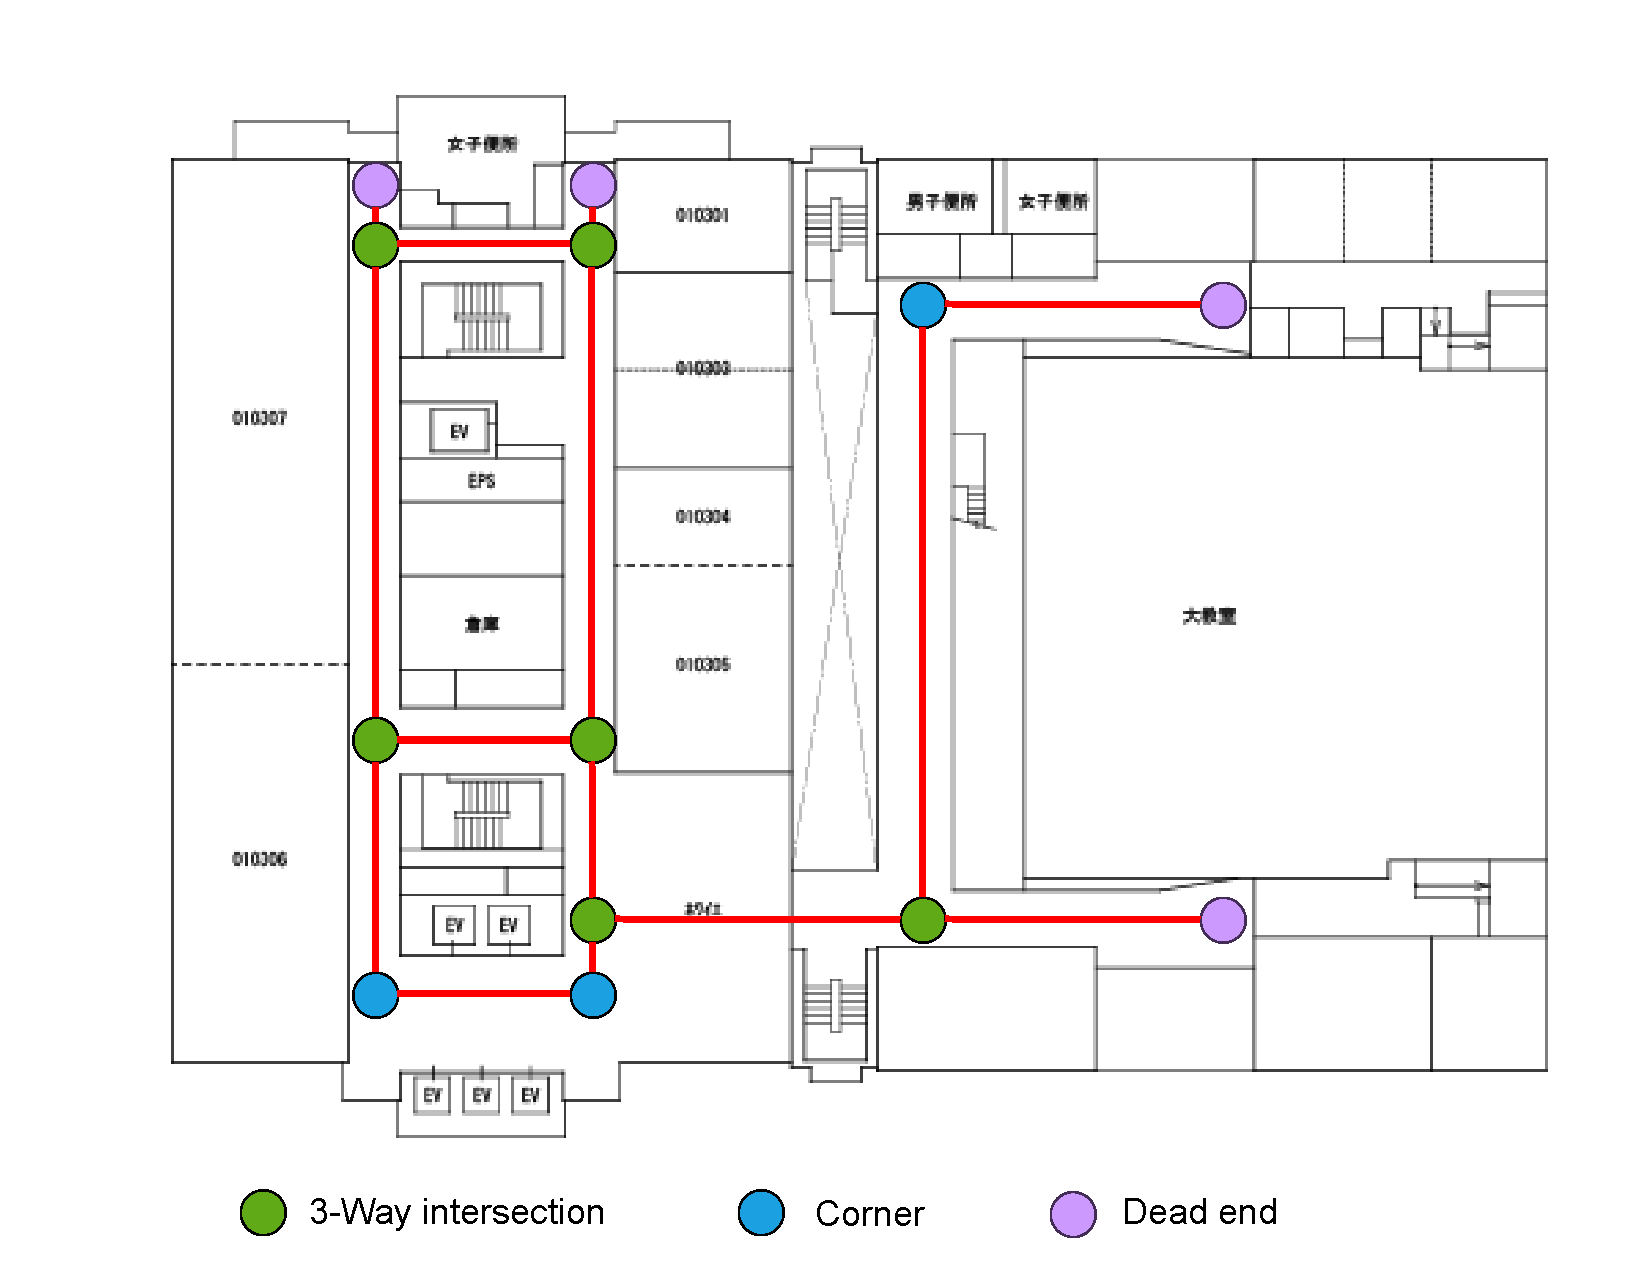
\includegraphics[width=130mm]{images/pdf/ishiguro/topo.pdf}
  \caption{Experimental environment}
  \label{fig:topo}
\end{figure}

\subsection{シナリオの選定}
実験では島田ら用いた50例の中から,28例を選定した.
選定するにあたって,以下の条件を設定した.

\begin{enumerate}
  \item [1)] ロボットが移動困難な\figref{fig:cit3f}に示す部分を走行ルートに含まれないこと.
  \item [2)] 経路追従モジュールができない,「後ろを向く」などのその場での旋回が含まれていないこと.
  \item [3)] 通路の分類が困難な\figref{fig:cit3f}に示す部分が走行ルートが含まれないこと.
\end{enumerate}

\begin{figure}[htbp]
  \centering
  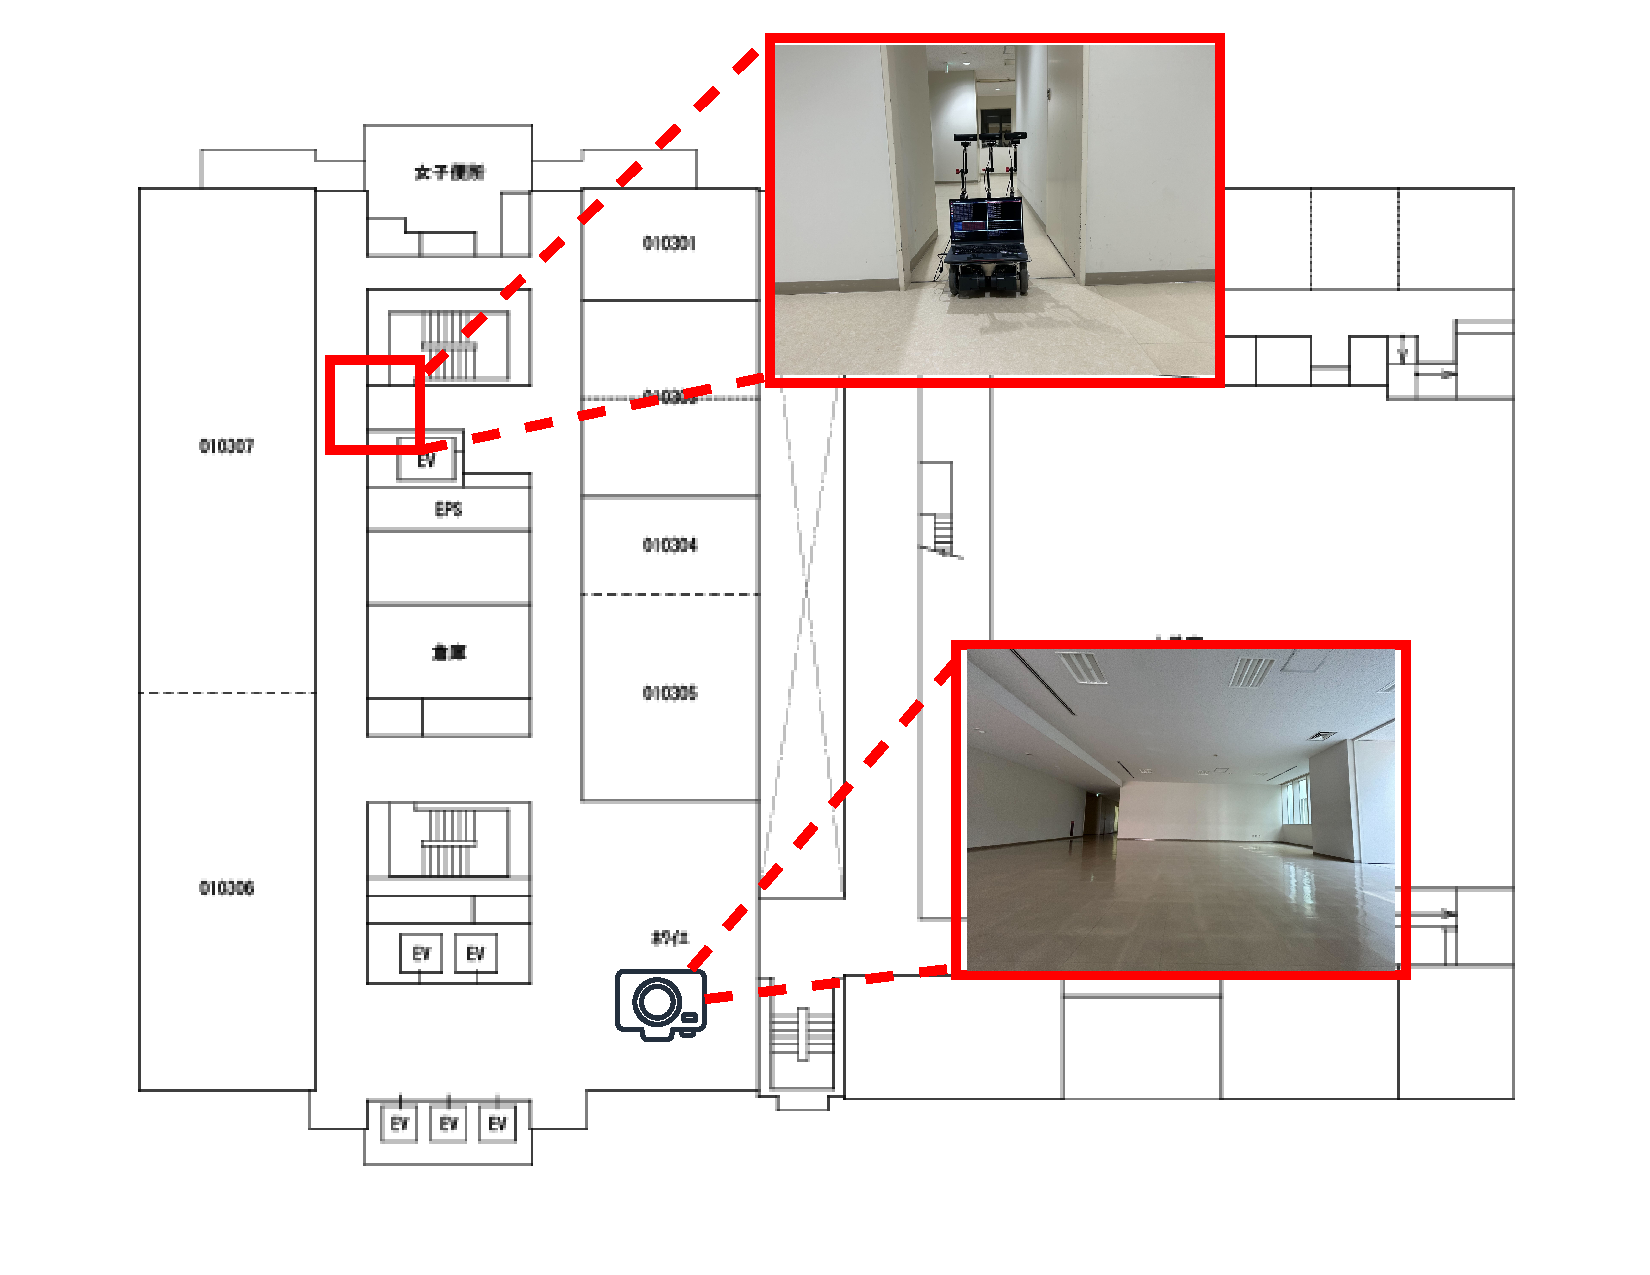
\includegraphics[width=130mm]{images/pdf/ishiguro/cit3f.pdf}
  \caption{Experimenta}
  % \label{fig:topo}
\end{figure}

\subsection{経路追従モジュールの訓練}
\figref{}に示すルートをオンライン学習させながら1週走行する.
オンライン学習で作成したモデルに追加でオフライン学習を行う.
オフライン学習時のデータセットはオンライン学習の際に作成した1週分のデータを用いる.
データセットからはオンライン学習と同様のバッチサイズ8で画像をランダムに取得し,epoch数は20とした.

\subsection{通路分類モジュールの訓練}
\figref{}に示すルートをROS の navigation パッケージを使用して,経路を1周する.
その際,3つのカメラからそれぞれ画像データを収集しながら走行する.
学習時のパラメータとして,バッチサイズ32,epoch数30とし,コストアプローチに用いた重みは~~~に示す.

\subsection{シナリオに基づくナビゲーション}
2 つのモジュールを訓練後,ロボットが目的地まで到達できるか確認する.
実験では,ロボットをシナリオのスタート地点,向きに配置し,シナリオを1例ずつ投入する.
途中で壁に衝突や,経路の選択を誤ることなく自律移動し,目的地で停止した際に成功とする.